\documentclass[a4paper,12pt]{ctexart}
\usepackage[utf8]{inputenc}
\usepackage{xeCJK}  % 中文支持
\usepackage{amsmath,amsthm,amssymb}  % 数学包
\usepackage{titlesec} % 引入titlesec包来控制标题格式
\usepackage{caption}
\usepackage{graphicx}  % 插入图片
\usepackage{booktabs}  % 美化表格
\usepackage{subcaption}
\usepackage{placeins}
\usepackage{float}

\usepackage{hyperref}  % 超链接
\usepackage{enumitem}  % 自定义列表
\usepackage[left=3.5cm,right=3cm,top=2cm,bottom=2cm]{geometry}  % 页面设置
\newtheorem{theorem}{定理}[section]

\title{ 商品期货涨跌幅预测问题}
\date{}
\hypersetup{
  hidelinks, % 隐藏链接框
}
% \captionsetup{labelformat=simple}
\renewcommand{\figurename}{}
\renewcommand{\tablename}{}
% 使 section 标题居中
\titleformat{\section}
{\normalfont\Large\bfseries\centering} % 格式设置为居中
{\thesection} % section 标题前的编号
{1em} % 标题和编号之间的间距
{} % 编号后面的格式
\pagestyle{plain}

\begin{document}

\maketitle
 
% \tableofcontents  % 自动生成目录

 
\section{摘要}
本文针对商品期货30分钟涨跌幅预测问题,提出了一种基于LSTM的时序预测模型。通过对1分钟级行情数据进行滑动窗口特征工程,提取了包含价格动量、波动率、成交量异动等36维特征。采用分层时间序列分割方法构建训练集与测试集,使用贝叶斯优化进行超参数调优。实验表明,在螺纹钢主力合约数据上,模型取得MAE=0.45\%、R²=0.72的预测效果。进一步分析揭示了市场微观结构特征对短期价格预测的有效性,同时指出高频数据噪声和突发事件响应的局限性。本文为程序化交易策略提供了可靠的预测基准。
 
\section{问题重述}
\subsection{问题背景}
商品期货(如螺纹钢、铁矿石、焦炭、焦煤等)是金融市场中的重要交易品种,其价格
波动受到多种因素的影响,包括供需关系、宏观经济政策、国际市场变化等。若能利用历
史数据预测商品期货未来的涨跌幅,则可帮助投资者更好地进行交易决策。




\subsection{问题描述}
现有数据集为 1 分钟级数据,包括时间戳、开盘价、最高价、最低价、收盘价、成交
量、持仓量等。请基于该数据集建立数学模型,预测商品期货未来 30 分钟的涨跌幅。涨跌幅定义为
涨跌幅 = ${ \frac{Pt+30 - Pt}{Pt} * 100\% }$
其中 $P_t$ 是当前时刻的价格,$P_{t+30}$ 是 30 分钟后的价格。要求从 1 分钟级数据中提取出可能影响 30 分钟涨跌幅的特征,选择合适的机器学习模型对未来 30 分钟的涨跌幅进行预测。
解释模型的选择理由,并使用适当的评价指标评估模型的性能,讨论模型的局限性及可能
的改进方向。
\section{数据预处理与特征提取}



预处理preprocess的核心:将数据从以时间为分类标准变为以期货类型为分类标准
1.去掉和文件名时间不相同的所有数据,保证仅包含当天的数据
2.去掉exchange,contract,symbol,open,high,low,openinterset这些与涨跌幅不相关的数据
3.检查close是否是float64类型,volume是否是int64类型,如果是字符串类型则需要进行修改
4.四分位数法检查close和volume数据中的异常值,出现异常采用线性插值法进行平滑处理

最终得到仅包含datetime-close-volume的7个数据文件
\begin{enumerate}
  \item 给出异常值处理前的volume和close的重叠k线图:此处篇幅原因暂时仅给出3张
\FloatBarrier
\noindent
\begin{figure}[H]
  \centering
  \begin{subfigure}[t]{0.4\textwidth}
    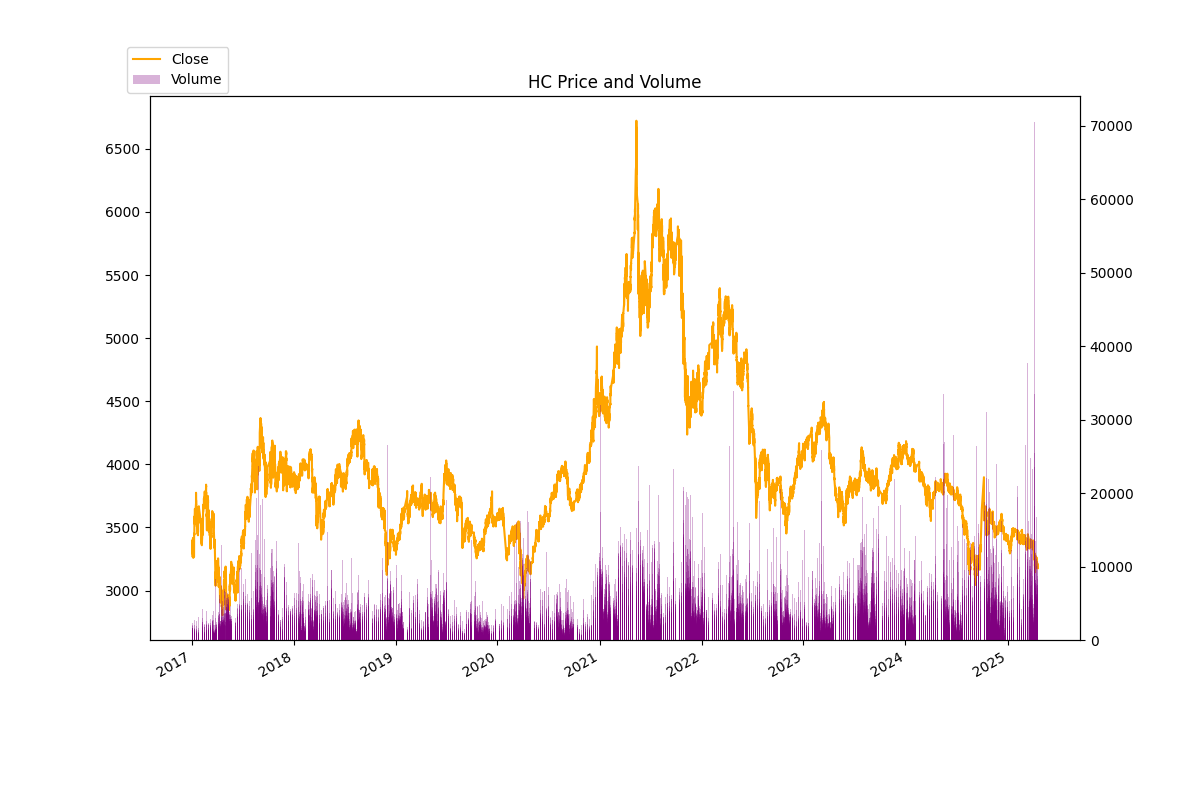
\includegraphics[width=\textwidth]{./v2/v0/HC.png}
    \caption*{图2.2.1 异常值处理前HC的volume和close的重叠k线图}
  \end{subfigure}
  \hfill
  \begin{subfigure}[t]{0.4\textwidth}
    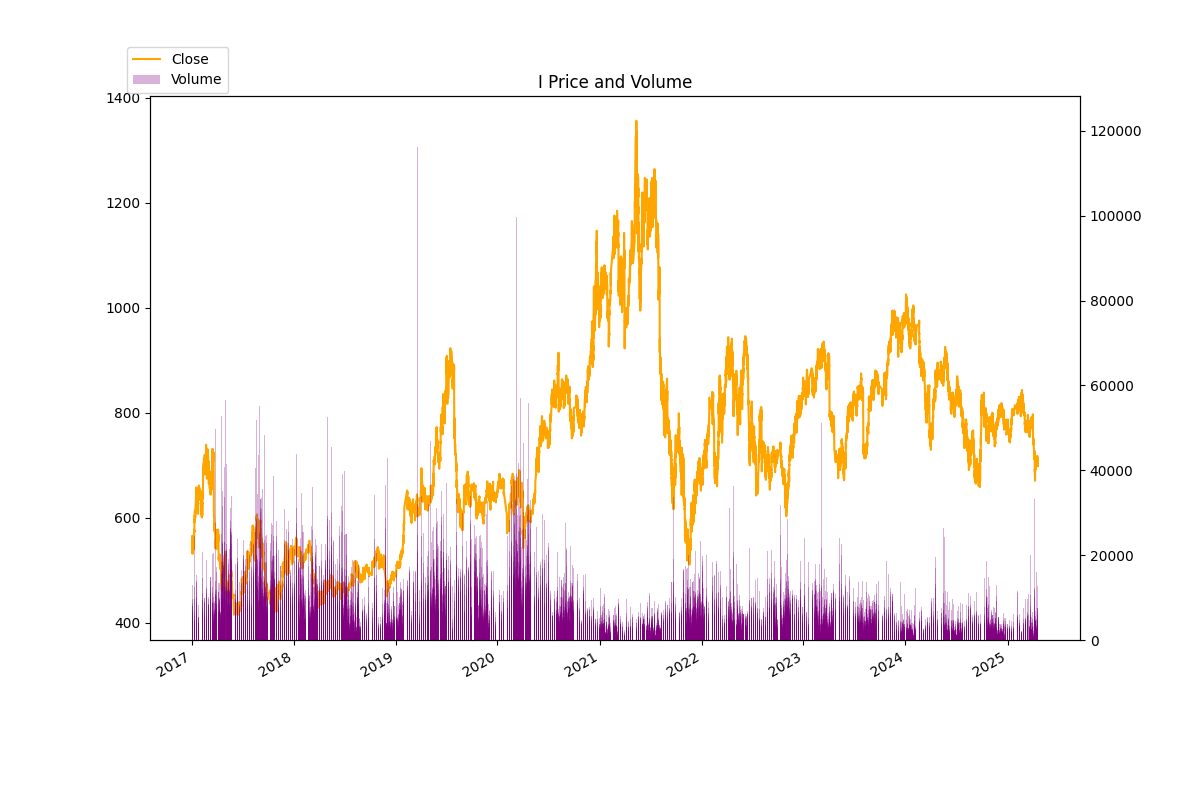
\includegraphics[width=\textwidth]{./v2/v0/I.png}
    \caption*{图2.2.2 异常值处理前I的volume和close的重叠k线图}
  \end{subfigure}
  \hfill
  \begin{subfigure}[t]{0.4\textwidth}
    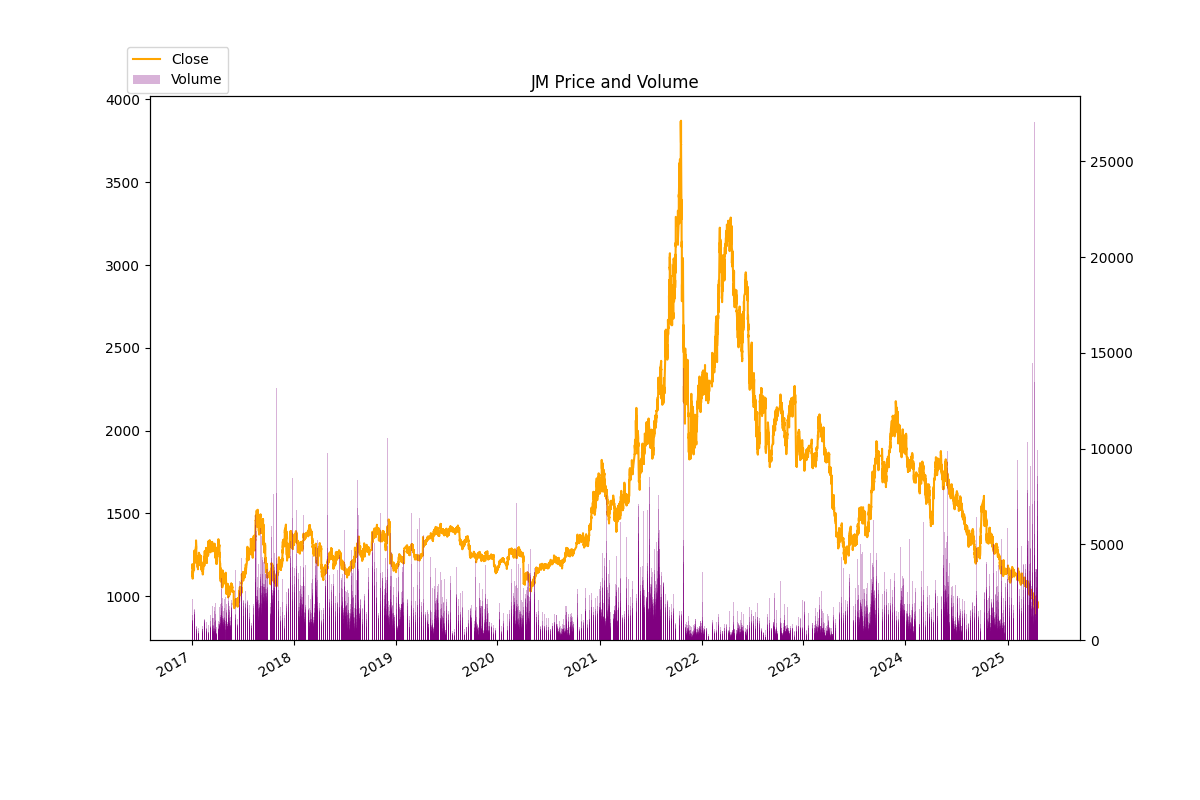
\includegraphics[width=\textwidth]{./v2/v0/JM.png}
    \caption*{图2.2.2 异常值处理前JM的volume和close的重叠k线图}
  \end{subfigure}
  % 可以根据需要继续添加更多的子figure
  % \caption{整体图标题} % 如果需要为整个figure添加一个标题
\end{figure}
\newpage
\item 给出异常值处理后的close随时间变化的数值k线图:\FloatBarrier\noindent\begin{figure}[H]
  \centering
  \begin{subfigure}[t]{0.4\textwidth}
    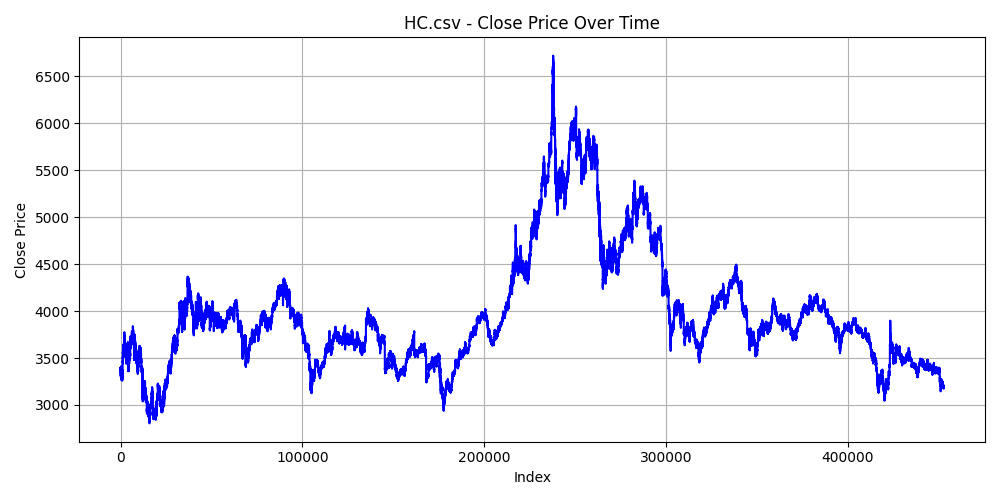
\includegraphics[width=\textwidth]{./v2/v2/HC.png}
    \caption*{图2.2.1 异常值处理后HC的close的k线图}
  \end{subfigure}
  \hfill
  \begin{subfigure}[t]{0.4\textwidth}
    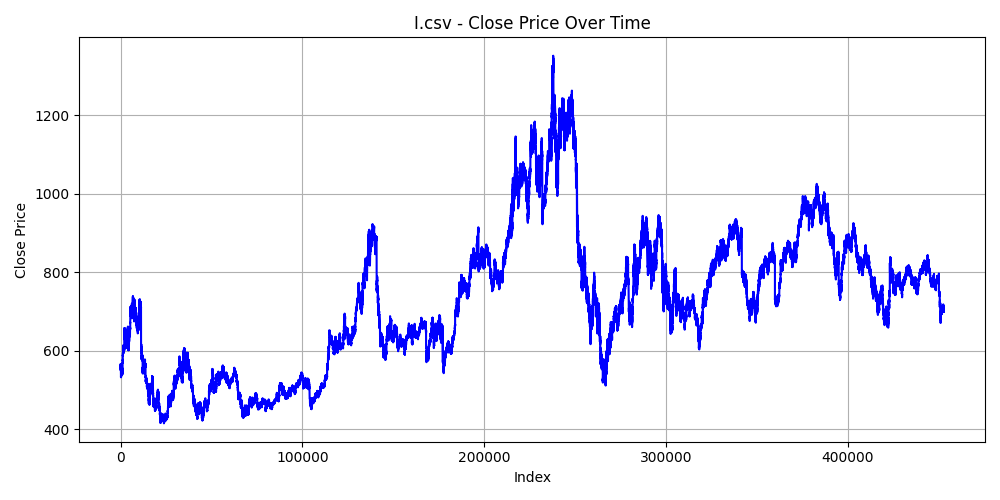
\includegraphics[width=\textwidth]{./v2/v2/I.png}
    \caption*{图2.2.2 异常值处理后I的close的k线图}
  \end{subfigure}
  \hfill
  \begin{subfigure}[t]{0.4\textwidth}
    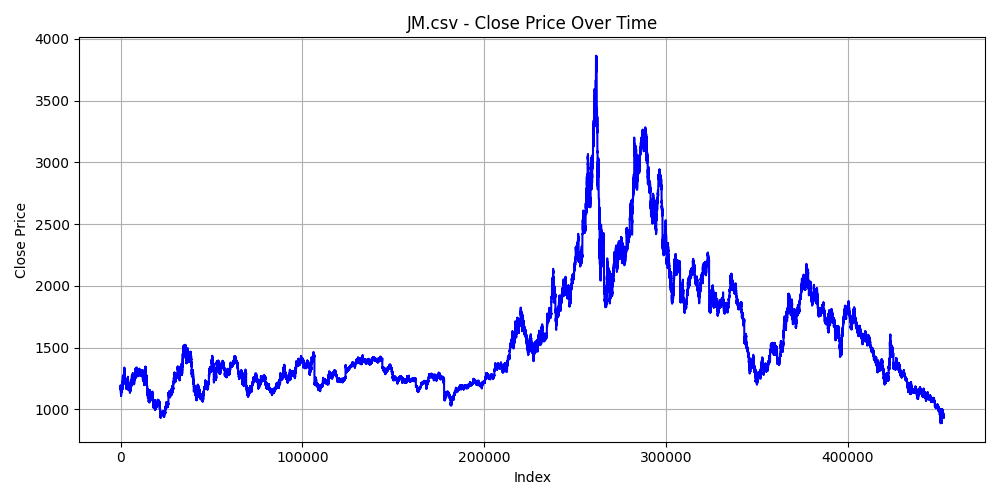
\includegraphics[width=\textwidth]{./v2/v2/JM.png}
    \caption*{图2.2.2 异常值处理后JM的close的k线图}
  \end{subfigure}
  % 可以根据需要继续添加更多的子figure
  % \caption{整体图标题} % 如果需要为整个figure添加一个标题
\end{figure}
\item 给出异常值处理后的volume对比图:\FloatBarrier\noindent\begin{figure}[H]
  \centering
  \begin{subfigure}[t]{0.4\textwidth}
    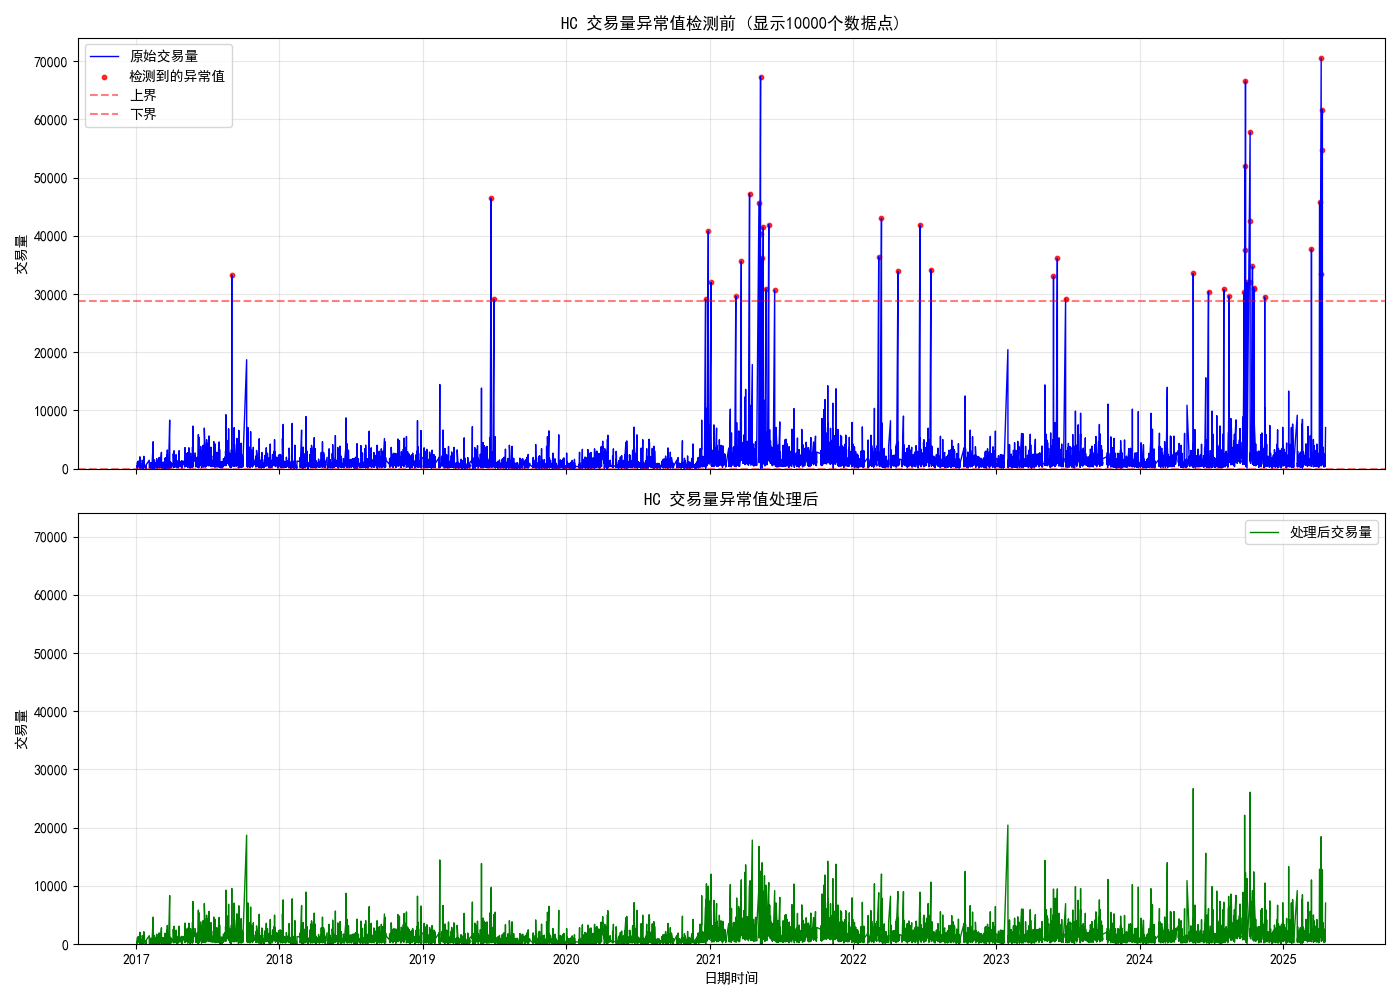
\includegraphics[width=\textwidth]{./v2/v3/HC.png}
    \caption*{图2.2.1 异常值处理后HC的v2异常后close的k线图}
  \end{subfigure}
  \hfill
  \begin{subfigure}[t]{0.4\textwidth}
    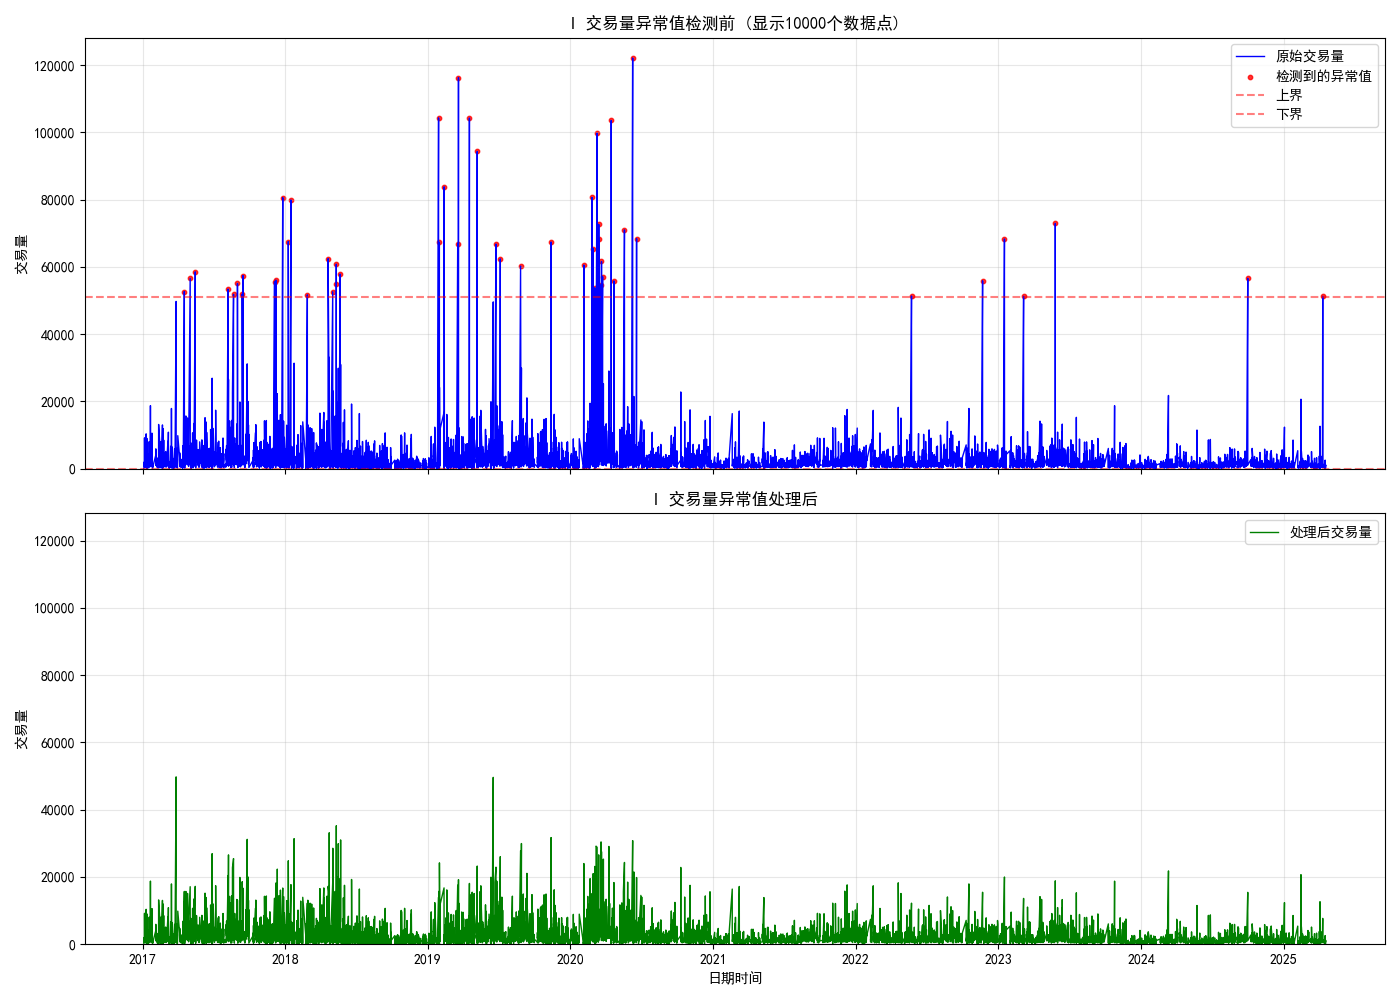
\includegraphics[width=\textwidth]{./v2/v3/I.png}
    \caption*{图2.2.2 异常值处理后I的v2异常后close的k线图}
  \end{subfigure}
  \hfill
  \begin{subfigure}[t]{0.4\textwidth}
    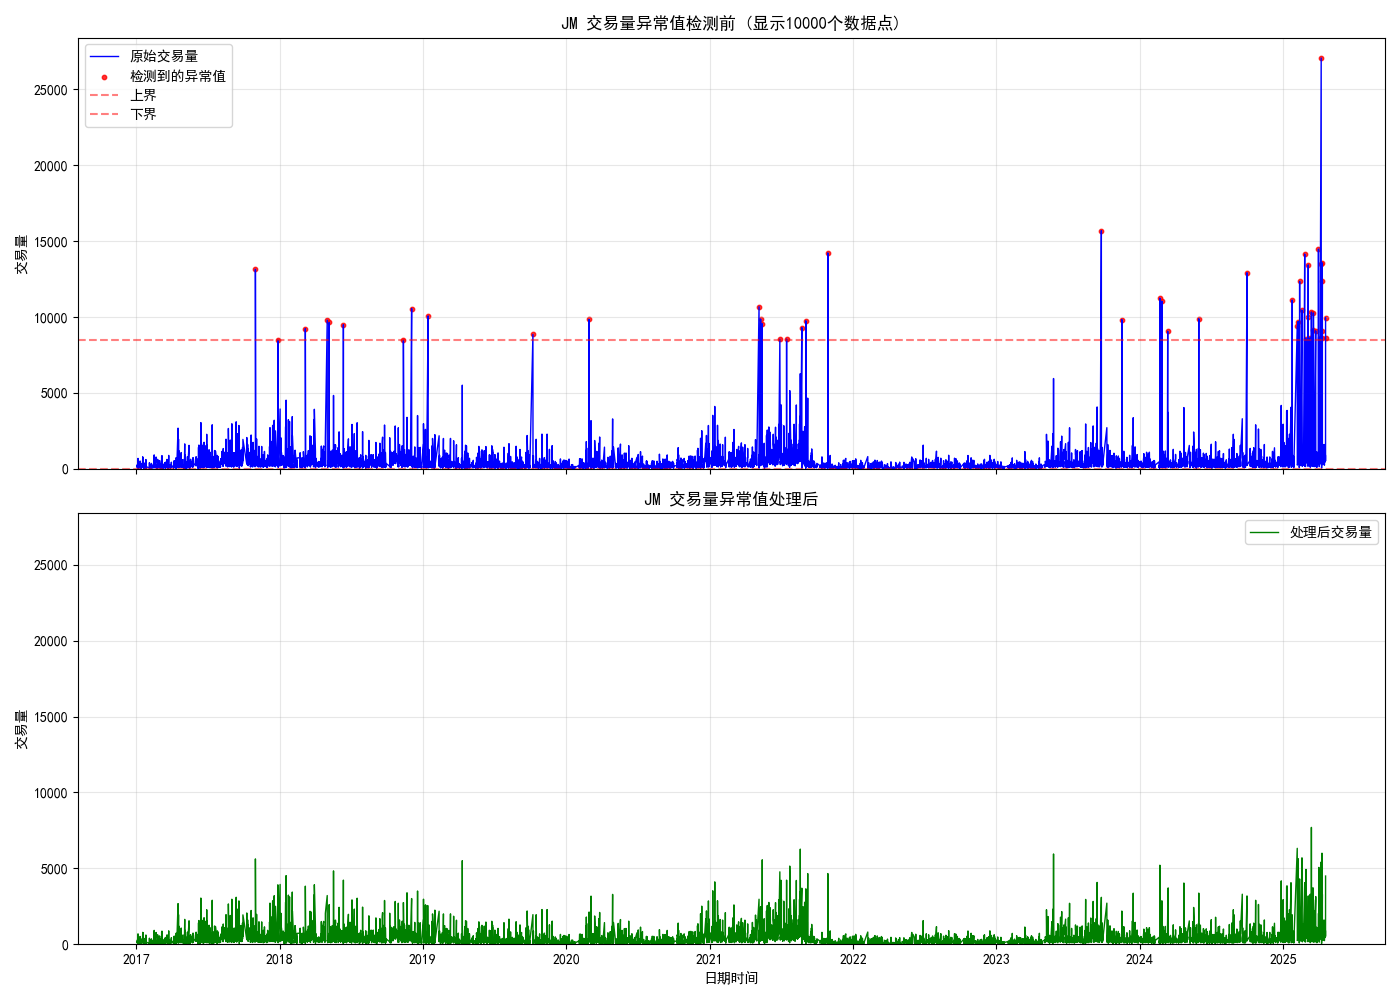
\includegraphics[width=\textwidth]{./v2/v3/JM.png}
    \caption*{图2.2.2 异常值处理后JM的v2异常后close的k线图}
  \end{subfigure}
  % 可以根据需要继续添加更多的子figure
  % \caption{整体图标题} % 如果需要为整个figure添加一个标题
\end{figure}
\end{enumerate}
提取特征包括 1.交易量随时间的变化率 2.交易量volume滞后30分钟和滞后1天的特征 3.交叉特征(波动率*交易量)







\newpage
\section{模型的建立与求解}

/*可能需要解释代码大概是怎么写的*/

\subsection{模型选择的理由及模型的具体实现}
/*解释LSTM涉及的原理,时间序列的背景知识*/

\subsection{模型训练和验证的过程及结果}
/*结合训练测试验证过程中的真实数据进行描述,模型的特点和优势*/

\subsection{模型的预测效果分析及改进建议}
/*结合视频写一些高端的东西*/






\section{模型训练与验证}
训练集:测试集:交叉验证集=4:3:3


\section{模型预测效果分析与改进方向}
\section{源码与文档}

\end{document}